%!TEX root = paper.tex

\section{The Spack Package Manager}
\label{sec:implementation}
Based on our experiences at LLNL, we have developed
{\it Spack}, the Supercomputing PACKage manager.
Spack is written in Python.  We chose Python because it is
very widely used int he HPC community, and because it provides
flexible scripting capabilities. 
%
Like some prior systems, Spack supports arbitrarily many software installations.
It borrows ideas from Nix; packages are installed in their own prefixes,
and configurations are managed using hashes.
% 
Spack adds several unique capabilities that are essential for HPC:
\begin{enumerate}
\item {\bf Parametric builds} address the matrix problem:
      Packages are parameterized by name, version, architecture, compiler, 
      options, and dependencies.
\item To manage the configuration space, spack provides a novel, 
      recursive {\bf spec syntax} for dependency graphs.
\item Specs support versioned, ABI-incompatible interfaces like MPI through
      {\bf versioned virtual dependencies}.
\item Spack builds with {\bf compiler wrappers} that reduce the burden of build
      consistency on the package author.
\end{enumerate}


%!TEX root = paper.tex

\subsection{Packages}

%\subsubsection{Package Files}
\begin{figure}
	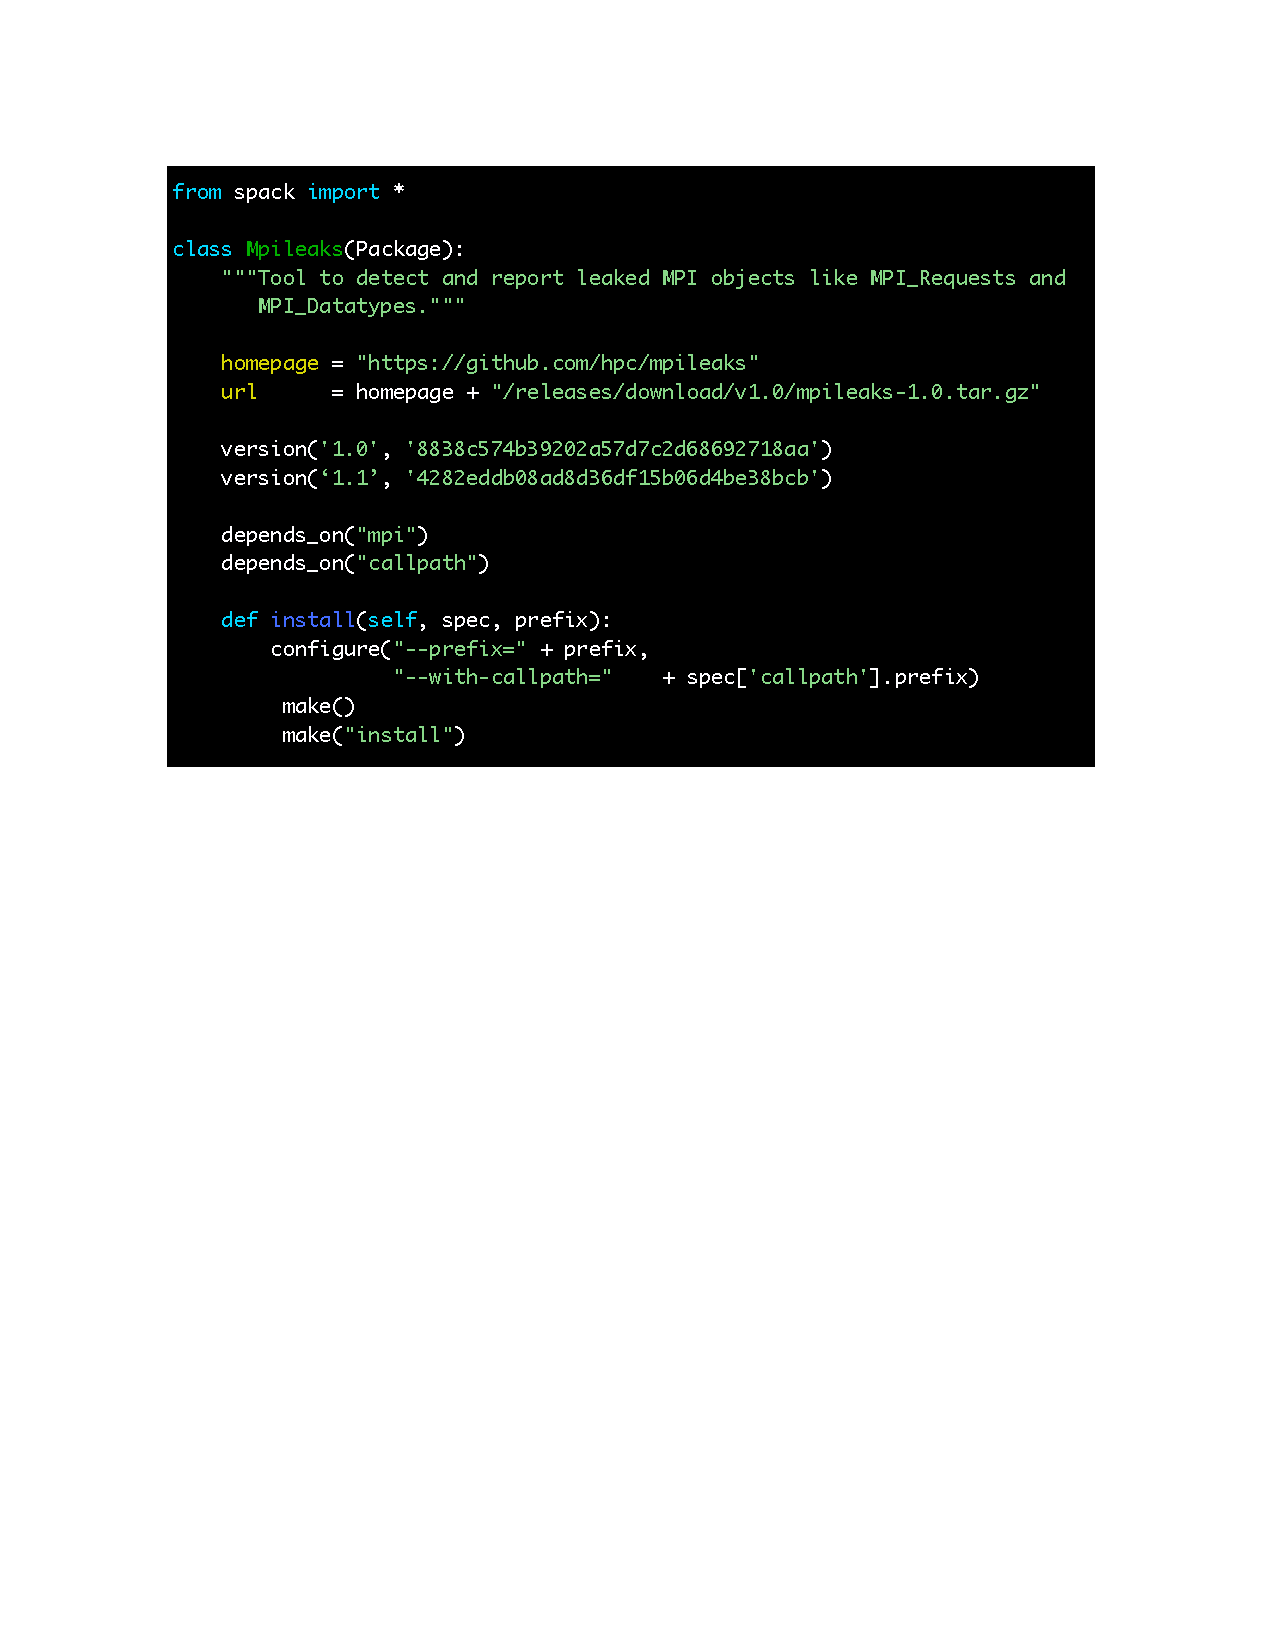
\includegraphics[width=\columnwidth]{code/mpileaks.pdf}
	\caption{
		Spack package for the {\tt mpileaks} tool.
		\label{fig:mpileaks}
	}
\end{figure}

In Spack, packages are build scripts that describe how to build software
artifacts.  Each package is a class written in pure Python to describe
{\it specific} build instructions, and it must extend the {\tt Package}
base class, which implements the more general parts of the build process.
Spack implements a simple, embedded domain-specific language (DSL) to make
packaging easier; it adds special directives such as {\tt depends\_on} and
{\tt version} that add metadata to the class.

Figure~\ref{fig:mpileaks} shows the package for \mpileaks, an LLNL-developed
tool for finding leaks in MPI programs.
Inside the {\tt MpiLeaks} class, the package provides a text description
and a homepage, as well as 
a download URL.  Next, two {\tt version} directives identify known versions
of the package, and MD5 checksums ensure they can be downloaded safely.
Below this, two {\tt depends\_on}
directives indicate prerequisites that must be installed before \mpileaks.
Last, each package defines an {\tt install()} method, which contains the
commands used to build the package.  Spack's DSL allows shell
commands to be invoked as Python functions. Here, the {\tt install()} 
method invokes the familiar {\tt configure}, {\tt make}, and
{\tt make install} build commands, as a shell script would.







\subsection{Spack Specs}\label{sec:specs}

  Specs are partial descriptions of full
dependency graphs, but they are concise.  This allows a user to use
only a few parameters to quickly identify a configuration to install,
or to query existing installations and their dependencies.



\todo{1 page}



\subsection{Versioned Virtual Dependencies}
	\todo{.5 page}

\subsection{Abstract \& Concrete Specs}
	\todo{.75 page}
	

